In this chapter, we will discuss the obtained results in the process of firmware acquisition and firmware extraction, previous steps before the actual firmware re-hosting.

\section{Work Environment}

Before discussing our results, this section will explain how our team has set up our software work environment. A personal computer was configured with a virtualization solution called Proxmox Virtual Environment as operating system. Proxmox VE is a Linux operating system (based on Debian distribution) that act as a virtualization server. It provides an web interface in which the user can create and manage virtual machines. Proxmox VE uses the already mentioned QEMU \cite{qemu} (mentioned in Sections \ref{sec:re-hosting} and \ref{sec:qemu}) and the Linux KVM (Kernel Virtual Machine) technology as a backend, and provides a hypervisor for managing containers and virtual machines.

This setup allows us to easily create virtual machines to test software in an environment of isolation, save virtual machines disk snapshots and rollback in time if needed. A main guest virtual machine with Debian 10 was selected to host our main efforts. Table \ref{tab:vm-specs} shows the specifications of the machines (host and virtual machine) used as our main work environment. The access to the machines was done using the SSH protocol.

\begin{table}[H]
\centering
\caption{Specifications for the host machine and main virtual machine used in our project.}
\begin{tabular}{ccc}
\hline
\textbf{Specifications} & \textbf{Host} & \textbf{Guest VM} \\ \hline
Operating System        & Proxmox VE           & Debian 10             \\
Kernel Version          & {\tt5.4.128-1-pve}   & {\tt 4.19.0-18-amd64} \\
CPU Model               & AMD Ryzen 5 2600     & {\tt kvm64}           \\
Number of Cores         & 6 Cores              & 4 Cores               \\
Number of Threads       & 12 Threads           & 4 Threads             \\
Memory                  & 32 GB                & 20 GB                 \\ \hline
\end{tabular}
\label{tab:vm-specs}
\end{table}

Furthermore, to enhance the experience when working connected to a remote machine using the SSH protocol, some tools were extensively used in our work. Just for the record, we will list here some of the utilities we used as this can help other people that work in similar environment, in which remote work via SSH protocol is a common practice.

\begin{itemize}
    \item \textbf{Tmux}: Utility to save SSH sessions. Using Tmux one can create a session inside the remote server. Sessions can be attached and detached, in a way that a person can leave processes running in a remote machine and end close the terminal running the SSH client, in a way that the running process will keep running in the remote machine. Afterwards, the user can simply join the remote Tmux session again and he will be reattached to the running processes he left in the session.
    
    \item {\tt ngrok}: This tool provides a way to easily open network tunnels to expose a service on the internet without requiring the user to forward ports to expose services in it's local network. The user can choose which protocol and port {\tt ngrok} will expose to the internet, and the tool will provide a URL that forwards internet connection to the local service the user has exposed. A daemon running {\tt ngrok} was configured in our guest VM allowing us to work on our server anywhere on the internet (outside our local network).
\end{itemize}

It's also worth mentioning that we also used the PostgreSQL database to save interesting data. Interaction with the database was done using the {\tt psql} command line tool.

\section{Jupyter Notebooks}

In order to organize work, specially as we intend to collaborate as a team and also to collaborate with external researchers, during our experiments, we felt the need to have a tool to help us record the experiments and to save the acquired information during the experimentation phase. Therefore, we decided a good fit for this need was to use Jupyter Notebooks as a way to report experiments and results. Jupyter Notebooks are a way to save documents containing formatted text (in markdown language) with snippets of code (in Python or shell scripts) and its respectively outputs.

Notebooks containing the code that was executed in order extract information from the firmware images and to produce the results shown on this paper can be found on this project repository \cite{github:c2dc-toso} together with the output produced by their execution. Figure \ref{fig:jupyter} shows the interface of one of the implemented Jupyter notebooks.

\begin{figure}[H]
    \centering
    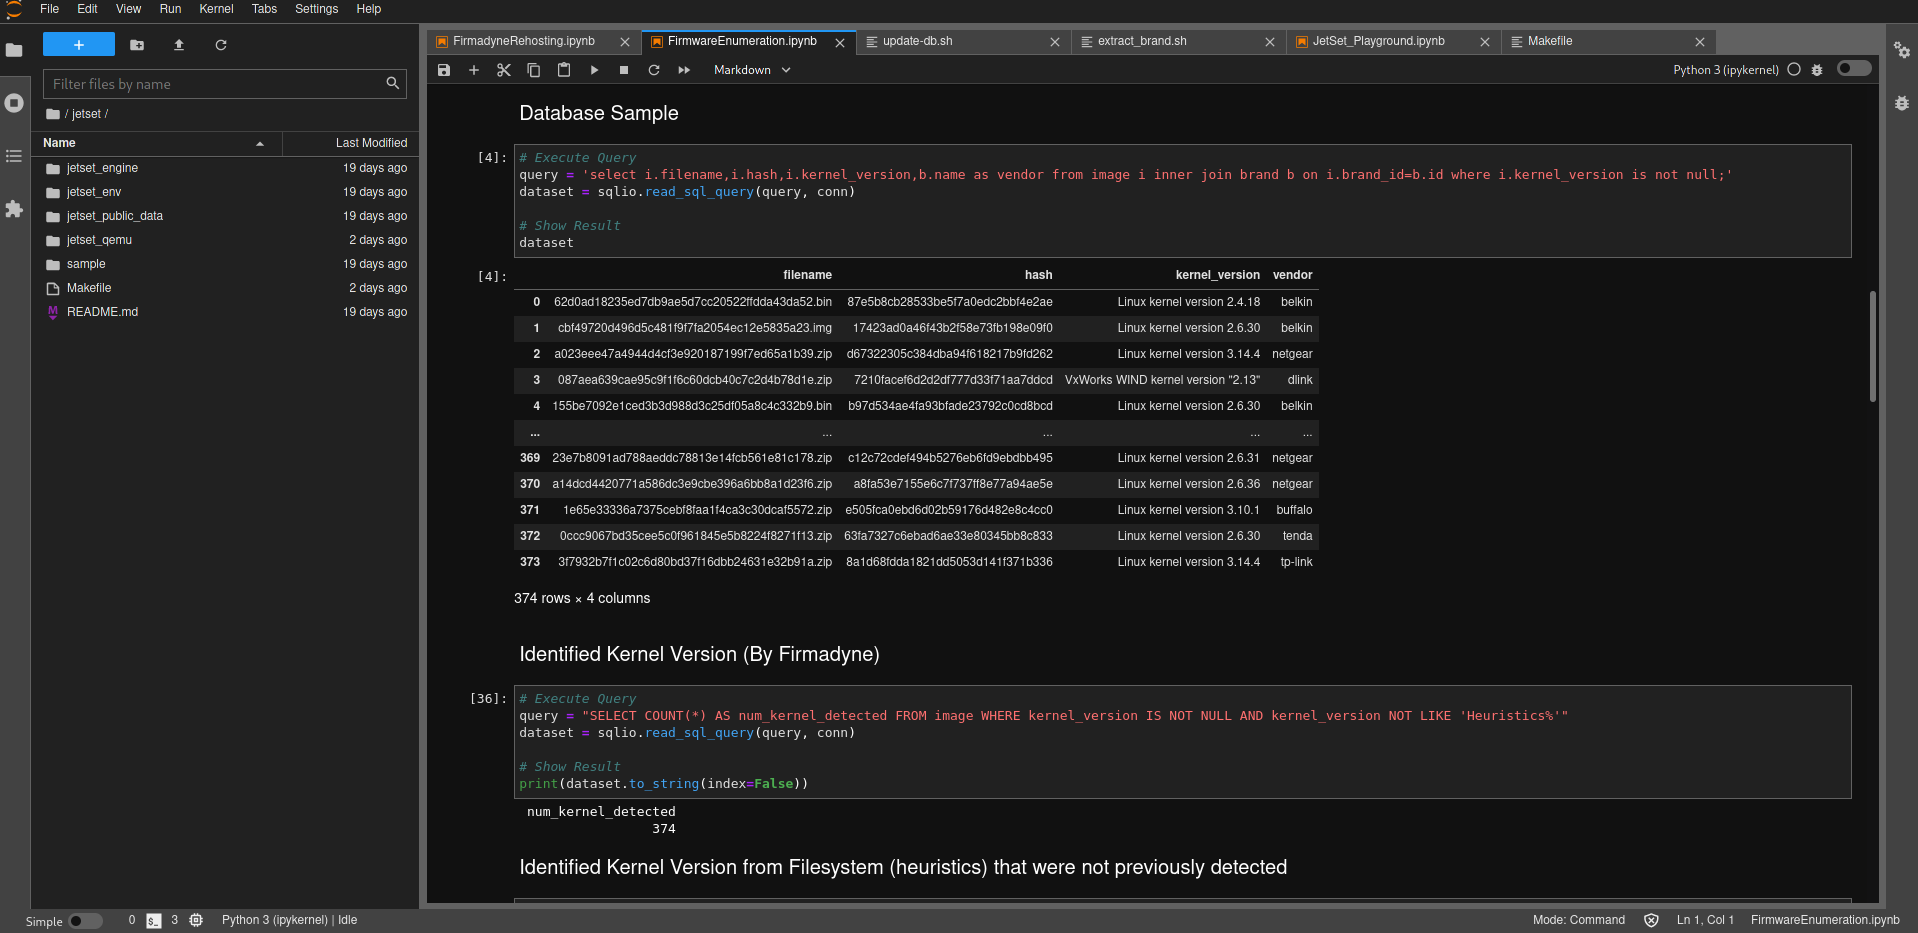
\includegraphics[width=1.0\textwidth]{figs/jupyter.png}
    \caption{Jupyter Notebook interface (showing firmware enumeration notebook).}
    \label{fig:jupyter}
\end{figure}

\section{Firmware acquisition}
\label{sec:firmware-aquisition}

For the firmware acquisition, we used a fork of the Firmadyne's \cite{firmadyne} original scraper \cite{github:scraper}. This modified scraper version has fixed some compatibility issues the original scraper has with Python 3 and also updates the spiders to match more updated version of vendor websites. Without modifying any of the spiders provided by the scraper, we executed the scraper to automatically find and download firmware from all the possible vendors implemented by the scraper.

As the project is part of a team research, and to facilitate the research setup between different machines, we also implemented a script to automate the execution of the scraper and to enumerate the scraped firmware images for each vendor.

In total, 9176 firmware images were downloaded throughout this process. Table \ref{tab:scraper} show the amount of firmware images and its combined file size for each vendor.

\begin{table}[H]
\centering
\caption{Downloaded firmware images per vendor.}
\begin{tabular}{ccc}
\hline
\textbf{Vendor} & \textbf{Firmware Images} & \textbf{Combined File Size} \\ \hline
OpenWrt         & 3898                     & 15 GB                       \\ 
Netgear         & 1544                     & 48 GB                       \\ 
MikroTik        & 873                      & 11 GB                       \\ 
TP-Link         & 788                      & 7.2 GB                      \\ 
D-Link          & 591                      & 8.8 GB                      \\ 
Polycom         & 547                      & 136 GB                      \\ 
Tomato (Shibby) & 321                      & 2.3 GB                      \\ 
QNAP            & 279                      & 43 GB                       \\ 
Tenda           & 176                      & 825 MB                      \\ 
Ubiquiti        & 78                       & 2.3 GB                      \\ 
Belkin          & 36                       & 267 M                       \\ 
Mercury         & 33                       & 25 MB                       \\ 
pfSense         & 6                        & 2.2 GB                      \\ 
Buffalo         & 6                        & 75 MB                       \\ \hline

\end{tabular}
\label{tab:scraper}
\end{table}

Note that the scraper also download firmware images from the OpenWrt project, which aims to develop a highly extensible GNU/Linux distribution suited for embedded devices (specially wireless routers). Because OpenWrt is not really a wireless router manufacturer, in the next statistics regarding the firmware images, the OpenWrt will be considered apart.

As the goal of this work is towards the process of re-hosting, this amount of firmware images is already enough for initial experiments with automated re-hosting. In further work, more vendors pages can be extracted, and we can update scraper's spiders if we judge there is need for a larger volume of firmware images. Also, just for the record, one of our contributors has already implemented a spider to acquire firmware from a vendor that is not contemplated on the original scraper list (ASUS), but this implemented spider was posterior to our data acquisition and thus it was not used for the results in this paper.

\section{Firmadyne Automation}

Although Firmadyne~\cite{firmadyne} has already implemented code to perform firmware acquisition (with the scraper), extraction and re-hosting, there is no code that integrates and automated these actions - at least in the code provided by Firmadyne's repository. In this sense, we implemented a lot of shell scripts to automate the execution of Firmadyne's atomic actions. More than that, in our Jupyter notebooks, we show code to automate steps from Firmadyne execution and to programmatically extract important data and statistics from the firmware directory and Firmadyne's original database.

Also, to better understand the tool, there was a lot of reverse engineering and 

\section{Firmware extraction}
\label{sec:firmware-extraction}

Firmware extraction was heavily based on the usage of the {\tt binwalk} tool, whose usage was wrapped inside a script provided by Firmadyne \cite{firmadyne}. This script, when executed with a firmware image as a parameter, recursively tries to extract files using {\tt binwalk} for this purpose. It defines a breadth and depth limit to this recursion strategy. During the extraction process, the script then tries to identify if any of the extracted directories has a Linux root directory structure (i.e. has {\tt /bin}, {\tt /etc}, {\tt /usr} directories and so on). If that is the case, then this filesystem structure is compressed and stored in a separate location (also defined as a parameter to the script). 21.48\% of the total amount of firmware files (1971 from 9176 images) were successfully extracted by Firmadyne's \cite{firmadyne} extraction script. Of these extracted images, 97.21\% (1916 images) had the root filesystem extracted and of these, 94.89\% (1818 images) had the architecture identified. Architecture identification is done by reading files in filesystem directories that should contain binary files (e.g. {\tt /bin} or {\tt /sbin}) and reading the header of these files.

Kernel detection is done by reading each entry identified by {\tt binwalk} in the extraction process and detecting known kernel types. These are also extracted and stored in a separate location. When using the script, the user has the option to disable kernel extraction, as this greatly improves execution speed since {\tt binwalk} spends a lot of effort in the extraction process. If kernel extraction is not disabled by user, then the script also tries to identify kernel version and store this information in Firmadyne's \cite{firmadyne} database if found.

When extracting firmware, if Firmadyne's extraction script is capable of identifying the original firmware filesystem, its structure (only the names of each files) is saved into a database, associating the files with the firmware id. After that the original filesystem (with files contents) is compressed and saved in an output folder. Therefore, it is easy to search for files inside the extracted firmware images as one can easily query the database to search for an specific filename. If the content of a file is desired, the associated compressed filesystem can be extracted to recover the desired file content.

As not all kernels are identified by the {\tt binwalk} tool during the extraction phase, we also developed an heuristic that uses regular expressions to search the extracted filesystem of each firmware image (querying the database) whose kernel was not identified during extraction and try to find directories that could reveal kernel version (e.g. {\tt /lib/modules/2.6.31} is an indicative that this image contains a 2.6.31 Linux kernel). This search is extremely fast compared to the filesystem extraction process and increased the number of kernel versions detected. Initially, with the Firmadyne's \cite{firmadyne} original extraction script, only 374 kernels were identified amongst the 1971 (18.98\%) of the total amount of firmware images. After running the described heuristics to determine kernel version from filesystem, the number of identified kernels increased to 1812 (384.49\% greater).

When considering only the firmware files with root filesystem extracted and architecture identified, 97.85\% (1779 images) had the kernel identified. That is, 1779 firmware images of our dataset had it's complete tuple identification: Architecture, Kernel Version and Root Filesystem. Figure \ref{fig:stats-funnel} shows the funnel of success for firmware extraction and illustrates the statistics just described.

\begin{figure}[H]
    \centering
    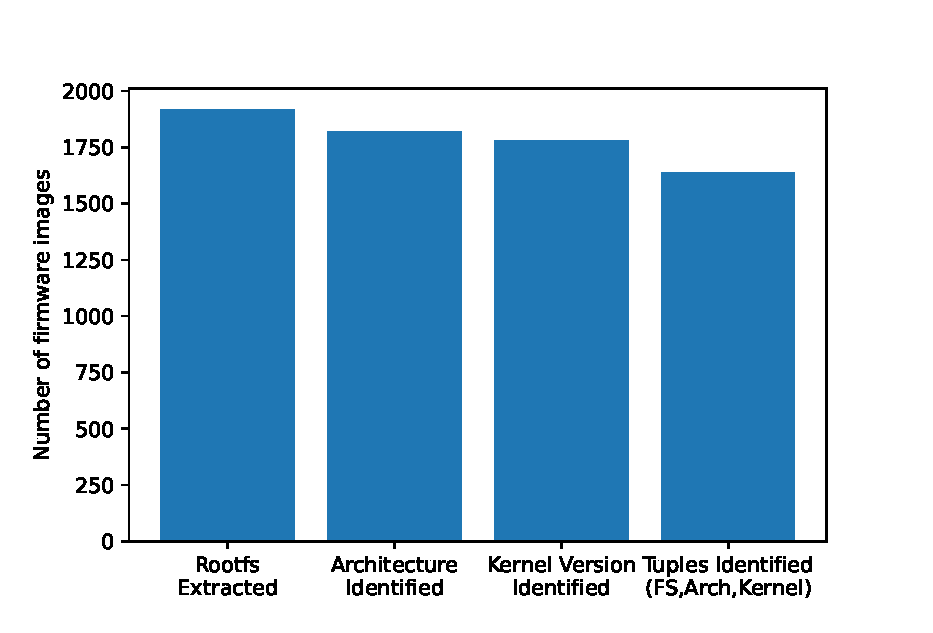
\includegraphics[width=0.90\textwidth]{figs/extraction_funnel.eps}
    \caption{Success funnel for firmware image extraction.}
    \label{fig:stats-funnel}
\end{figure}


It was also identified two issues in the extraction process. Some kernel image media types (formerly known as MIME types) were incorrectly identified as a type that was on the extraction script blacklist. This could be easily corrected excluding the identified type from the blacklist. The second issue is related to the recursive extraction process. The limits in breadth and depth exploration allow the {\tt binwalk} tool to have usable performance, but in some cases these limits were in fact responsible for the firmware extraction to be unsuccessful. Therefore, we believe using an heuristic to select files with the most potential to hold firmware kernel or filesystem to be extracted next. This way we can still have breadth and depth limits to maintain the extraction process feasible but it would also focus the extraction in files that are more prominent. This approach of using an heuristics although idealized was not yet implemented in our work.

Another enhancement we developed to the extraction process was the ability to extract addition kernel information. During kernel extraction, the kernel binary file is scanned for ASCII strings and from the result of this search we then extract kernel banner (a string containing kernel version, compiler version used during kernel compilation, compilation date and email of the developer who compiled the kernel) or identify for instance if the system being extracted refers to an OpenWrt Linux. These additional pieces of information are also stored in Firmadyne's \cite{firmadyne} database, that had its schema altered to contain a new column to store the extra information for a given firmware image.

% Falar das estatísticas; Colocar tabela com as estatísticas

\subsection{Architecture and Kernel Statistics}

Regarding firmware extraction and feature identification, we collected some statistics that may help the following steps of this work in kernel compilation and firmware re-hosting. Table \ref{tab:arch-stats} shows the amount of firmware images detected for each architecture identified when not considering the OpenWrt acquired firmware images. Also Tables \ref{tab:kernel-stats} and \ref{tab:kernel-family-stats} shows the five most common kernel versions and kernel families respectively when not considering OpenWrt, Tomato (Shibby) and pfSense. Finally, Tables \ref{tab:arch-stats-openwrt}, \ref{tab:kernel-stats-openwrt} and \ref{tab:kernel-family-stats-openwrt} shows the architecture, kernel version and kernel family statistics when also considering the OpenWrt, Tomato (Shibby) and pfSense firmware images.

The decision to include statistics with and without the aforementioned vendors firmware images takes in consideration the fact that the three names represent open projects and they may not represent firmware statistics that are aligned with the firmware in commercial products. For instance, OpenWrt is a project led by the community to develop a GNU/Linux firmware that could easily be extended by developers and act as a framework for developing applications for embedded devices. In the project's official documentation it is stated that ``\textit{In practice, this means that you can have all the features you need with none of the bloat, powered by a Linux kernel that's more recent than most other distributions.}'', which means that by design OpenWrt kernel version statistics might not be befitting other vendor's statistics.

\begin{table}[H]
\centering
\caption{Number of images identified for each found architecture without considering OpenWrt, Tomato and pfSense firmware images.}
\begin{tabular}{cc}
\hline
\textbf{Architecture}       & \textbf{Quantity of Images} \\ \hline
{\tt mipseb}                &  300                        \\ 
{\tt mipsel}                &  197                        \\ 
{\tt armel}                 &  182                        \\ 
{\tt ppceb}                 &   83                        \\ 
{\tt intelel}               &   69                        \\ 
{\tt intel64el}             &    4                        \\ 
{\tt mips64eb}              &    4                        \\ \hline
\end{tabular}
\label{tab:arch-stats}
\end{table}

\begin{table}[H]
\centering
\caption{Five most common kernel versions found in extracted firmware images without considering OpenWrt, Tomato and pfSense firmware images.}
\begin{tabular}{cc}
\hline
\textbf{Kernel Version} & \textbf{Quantity of Images} \\ \hline
3.3.5                  & 546                 \\
2.6.36                 &  59                 \\
2.6.31                 &  52                 \\
2.6.22                 &  48                 \\
3.3.8                  &  27                 \\ \hline
\end{tabular}
\label{tab:kernel-stats}
\end{table}

\begin{table}[H]
\centering
\caption{Five most common kernel families found in extracted firmware images without considering OpenWrt, Tomato and pfSense firmware images.}
\begin{tabular}{cc}
\hline
\textbf{Kernel Family} & \textbf{Quantity of Images} \\ \hline
3.3                     & 573                \\ 
2.6                     & 223                \\ 
3.10                    &  32                \\ 
3.14                    &  28                \\ 
3.6                     &  22                \\ \hline
\end{tabular}
\label{tab:kernel-family-stats}
\end{table}

% ===============================================================================================================

\begin{table}[H]
\centering
\caption{Number of images identified for each found architecture (also considering OpenWrt, Tomato and pfSense firmware images).}
\begin{tabular}{cc}
\hline
\textbf{Architecture}       & \textbf{Quantity of Images} \\ \hline
{\tt mipseb}                & 688                         \\ 
{\tt mipsel}                & 660                         \\ 
{\tt armel}                 & 303                         \\ 
{\tt ppceb}                 & 90                          \\ 
{\tt intelel}               & 69                          \\ 
{\tt intel64el}             & 4                           \\ 
{\tt mips64eb}              & 4                           \\ \hline
\end{tabular}
\label{tab:arch-stats-openwrt}
\end{table}

\begin{table}[H]
\centering
\caption{Five most common kernel versions found in extracted firmware images (also considering OpenWrt, Tomato and pfSense firmware images).}
\begin{tabular}{cc}
\hline
\textbf{Kernel Version} & \textbf{Quantity of Images} \\ \hline
5.4.14                  & 619                \\
3.3.5                   & 546                \\
2.6.22                  & 207                \\
2.6.36                  & 79                 \\
2.6.31                  & 52                 \\ \hline
\end{tabular}
\label{tab:kernel-stats-openwrt}
\end{table}

\begin{table}[H]
\centering
\caption{Five most common kernel families found in extracted firmware images (also considering OpenWrt, Tomato and pfSense firmware images).}
\begin{tabular}{cc}
\hline
\textbf{Kernel Family} & \textbf{Quantity of Images} \\ \hline
5.4                    & 658                \\ 
3.3                    & 573                \\ 
2.6                    & 402                \\ 
2.4                    & 37                 \\ 
3.10                   & 32                 \\ \hline
\end{tabular}
\label{tab:kernel-family-stats-openwrt}
\end{table}

As the kernel version for a specific product is a manufacturer decision, the previous statistics are biased by the manufacturer we could extract the most number of firmware images. Therefore, Table \ref{tab:kernel-stats-by-vendor} provide the same previous statistics grouped by router vendor. The code implemented to extract the statistics shown here from the firmware database and the respective output can be viewed in the jupyter notebooks output appended in our project's GitHub repository~\cite{github:c2dc-toso}. 

\begin{table}[H]
\centering
\caption{Five most common kernel versions found in extracted firmware images by vendor.}
\resizebox{0.75\textwidth}{!}{\begin{tabular}{cccccc}
\hline

\multicolumn{6}{c}{\textbf{Vendor: OpenWrt} (670 kernels)}                                                                    \\
\textbf{Architecture} & \multicolumn{1}{c|}{\textbf{Quantity of Images}} & \textbf{Kernel Version} & \multicolumn{1}{c|}{\textbf{Quantity of Images}} & \textbf{Kernel Family} & \textbf{Quantity of Images}  \\ \hline
{\tt mipseb}            & \multicolumn{1}{c|}{295}             & 5.4.15                 & \multicolumn{1}{c|}{619}                           & 5.4                    & 659                         \\
{\tt mipsel}            & \multicolumn{1}{c|}{282}             & 5.4.15                  & \multicolumn{1}{c|}{34}                           & 5.10                    & 11                         \\
{\tt armel}             & \multicolumn{1}{c|}{87}              & 5.10.72                 & \multicolumn{1}{c|}{11}                           & 4.14                    & 1                          \\
{\tt ppceb}             & \multicolumn{1}{c|}{6}               & 5.4.87                  & \multicolumn{1}{c|}{5}                            &                         &                            \\
                        & \multicolumn{1}{c|}{}                & 4.14.12                 & \multicolumn{1}{c|}{1}                            &                         &                            \\ \hline

\multicolumn{6}{c}{\textbf{Vendor: MikroTik} (546 kernels)}                                                                    \\
\textbf{Architecture}  &  \multicolumn{1}{c|}{\textbf{Quantity of Images}} & \textbf{Kernel Version} & \multicolumn{1}{c|}{\textbf{Quantity of Images}} & \textbf{Kernel Family} & \textbf{Quantity of Images} \\ \hline
{\tt mipseb}            & \multicolumn{1}{c|}{157}                & 3.3.5                  & \multicolumn{1}{c|}{546}                           & 3.3                     & 546                       \\
{\tt armel}             & \multicolumn{1}{c|}{86}                 &                        & \multicolumn{1}{c|}{}                              &                         &                           \\
{\tt ppceb}             & \multicolumn{1}{c|}{81}                 &                        & \multicolumn{1}{c|}{}                              &                         &                           \\ 
{\tt mipsel}            & \multicolumn{1}{c|}{73}                 &                        & \multicolumn{1}{c|}{}                              &                         &                           \\ 
{\tt intelel}           & \multicolumn{1}{c|}{68}                 &                        & \multicolumn{1}{c|}{}                              &                         &                           \\ \hline

\multicolumn{6}{c}{\textbf{Vendor: Tomato (Shibby)} (202 kernels)}                                                                    \\
\textbf{Architecture} & \multicolumn{1}{c|}{\textbf{Quantity of Images}} & \textbf{Kernel Version} & \multicolumn{1}{c|}{\textbf{Quantity of Images}} & \textbf{Kernel Family} & \textbf{Quantity of Images} \\ \hline
{\tt mipsel}            & \multicolumn{1}{c|}{170}               & 2.6.22                  & \multicolumn{1}{c|}{159}                         & 2.6                     & 179                        \\
{\tt armel}             & \multicolumn{1}{c|}{19}                & 2.6.36                  & \multicolumn{1}{c|}{20}                          & 2.4                     & 23                         \\
                        & \multicolumn{1}{c|}{}                  & 2.4.37                  & \multicolumn{1}{c|}{12}                          &                         &                            \\
                        & \multicolumn{1}{c|}{}                  & 2.4.20                  & \multicolumn{1}{c|}{11}                          &                         &                            \\ \hline

\multicolumn{6}{c}{\textbf{Vendor: TP-Link} (110 kernels)}                                                                    \\
\textbf{Architecture} & \multicolumn{1}{c|}{\textbf{Quantity of Images}} & \textbf{Kernel Version} & \multicolumn{1}{c|}{\textbf{Quantity of Images}} & \textbf{Kernel Family} & \textbf{Quantity of Images} \\ \hline
{\tt mipseb}            & \multicolumn{1}{c|}{59}                & 2.6.36                  & \multicolumn{1}{c|}{35}                          & 2.6                     & 80                         \\
{\tt mipsel}            & \multicolumn{1}{c|}{23}                & 2.6.31                  & \multicolumn{1}{c|}{34}                          & 3.3                     & 17                         \\
{\tt armel}             & \multicolumn{1}{c|}{16}                & 3.3.8                   & \multicolumn{1}{c|}{17}                          & 3.10                    & 8                          \\
{\tt mips64eb}          & \multicolumn{1}{c|}{2}                 & 2.6.15                  & \multicolumn{1}{c|}{5}                           & 3.4                     & 2                          \\
{\tt ppceb}             & \multicolumn{1}{c|}{2}                 & 3.10.14                 & \multicolumn{1}{c|}{3}                           & 3.14                    & 2                          \\ \hline

\multicolumn{6}{c}{\textbf{Vendor: Netgear} (101 kernels)}                                                                        \\
\textbf{Architecture} & \multicolumn{1}{c|}{\textbf{Quantity of Images}} & \textbf{Kernel Version} & \multicolumn{1}{c|}{\textbf{Quantity of Images}} & \textbf{Kernel Family} & \textbf{Quantity of Images} \\ \hline
{\tt mipseb}              & \multicolumn{1}{c|}{33}               & 3.14.77                 & \multicolumn{1}{c|}{22}                          & 2.6                    & 60                          \\
{\tt armel}               & \multicolumn{1}{c|}{32}               & 2.6.31                  & \multicolumn{1}{c|}{17}                          & 3.14                   & 26                          \\
{\tt mipsel}              & \multicolumn{1}{c|}{30}               & 2.6.22                  & \multicolumn{1}{c|}{15}                          & 2.4                    & 9                           \\
{\tt mips64eb}            & \multicolumn{1}{c|}{2}                & 2.6.36                  & \multicolumn{1}{c|}{11}                          & 4.4                    & 2                           \\
                          & \multicolumn{1}{c|}{}                 & 2.6.15                  & \multicolumn{1}{c|}{10}                          & 3.6                    & 2                           \\ \hline

\multicolumn{6}{c}{\textbf{Vendor: Tenda} (88 kernels)}                                                                    \\
\textbf{Architecture} & \multicolumn{1}{c|}{\textbf{Quantity of Images}} & \textbf{Kernel Version} & \multicolumn{1}{c|}{\textbf{Quantity of Images}} & \textbf{Kernel Family} & \textbf{Quantity of Images} \\ \hline
{\tt mipsel}            & \multicolumn{1}{c|}{42}                & 2.6.22                 & \multicolumn{1}{c|}{28}                           & 2.6                     & 55                         \\
{\tt mipseb}            & \multicolumn{1}{c|}{17}                & 3.10.9                  & \multicolumn{1}{c|}{13}                          & 3.10                    & 16                         \\
{\tt armel}             & \multicolumn{1}{c|}{12}                & 2.6.36                  & \multicolumn{1}{c|}{12}                          & 3.3                     & 10                         \\
                        & \multicolumn{1}{c|}{}                  & 2.6.30                  & \multicolumn{1}{c|}{12}                          & 3.4                     & 3                          \\
                        & \multicolumn{1}{c|}{}                  & 3.3.8                   & \multicolumn{1}{c|}{10}                          & 4.9                     & 2                          \\ \hline

\multicolumn{6}{c}{\textbf{Vendor: Ubiquiti} (26 kernels)}                                                                    \\
\textbf{Architecture} & \multicolumn{1}{c|}{\textbf{Quantity of Images}} & \textbf{Kernel Version} & \multicolumn{1}{c|}{\textbf{Quantity of Images}} & \textbf{Kernel Family} & \textbf{Quantity of Images} \\ \hline
{\tt armel}             & \multicolumn{1}{c|}{20}                & 3.6.5                  & \multicolumn{1}{c|}{20}                           & 3.6                     & 20                         \\
{\tt mipsel}            & \multicolumn{1}{c|}{6}                 & 3.10.4                  & \multicolumn{1}{c|}{3}                           & 3.10                    & 5                          \\
                        & \multicolumn{1}{c|}{}                  & 3.10.1                  & \multicolumn{1}{c|}{2}                           & 4.4                     & 1                          \\
                        & \multicolumn{1}{c|}{}                  & 4.4.16                  & \multicolumn{1}{c|}{1}                           &                         &                            \\ \hline

\multicolumn{6}{c}{\textbf{Vendor: D-Link} (21 kernels)}                                                                    \\
\textbf{Architecture} & \multicolumn{1}{c|}{\textbf{Quantity of Images}} & \textbf{Kernel Version} & \multicolumn{1}{c|}{\textbf{Quantity of Images}} & \textbf{Kernel Family} & \textbf{Quantity of Images} \\ \hline
{\tt mipseb}            & \multicolumn{1}{c|}{6}                & 2.6.19                 & \multicolumn{1}{c|}{6}                           & 2.6                     & 16                         \\
{\tt armel }            & \multicolumn{1}{c|}{2}                & 2.6.18                  & \multicolumn{1}{c|}{5}                          & 3.4                     & 2                          \\
                        & \multicolumn{1}{c|}{}                 & 2.6.14                  & \multicolumn{1}{c|}{4}                          & 2.4                     & 2                          \\
                        & \multicolumn{1}{c|}{}                 & 3.4.25                  & \multicolumn{1}{c|}{2}                          & 3.10                    & 1                          \\
                        & \multicolumn{1}{c|}{}                 & 2.4.27                  & \multicolumn{1}{c|}{2}                          &                         &                            \\ \hline

\multicolumn{6}{c}{\textbf{Vendor: Belkin} (12 kernels)}                                                                    \\
\textbf{Architecture} & \multicolumn{1}{c|}{\textbf{Quantity of Images}} & \textbf{Kernel Version} & \multicolumn{1}{c|}{\textbf{Quantity of Images}} & \textbf{Kernel Family} & \textbf{Quantity of Images} \\ \hline
{\tt mipseb}            & \multicolumn{1}{c|}{7}                & 2.6.30                  & \multicolumn{1}{c|}{7}                          & 2.6                     & 11                         \\
{\tt mipsel}            & \multicolumn{1}{c|}{3}                & 2.6.22                  & \multicolumn{1}{c|}{3}                          & 2.4                     & 1                          \\
                        & \multicolumn{1}{c|}{}                 & 2.6.31                  & \multicolumn{1}{c|}{1}                          &                         &                            \\
                        & \multicolumn{1}{c|}{}                 & 2.4.18                  & \multicolumn{1}{c|}{1}                          &                         &                            \\ \hline

\multicolumn{6}{c}{\textbf{Vendor: Buffalo} (3 kernels)}                                                                    \\
\textbf{Architecture} & \multicolumn{1}{c|}{\textbf{Quantity of Images}} & \textbf{Kernel Version} & \multicolumn{1}{c|}{\textbf{Quantity of Images}} & \textbf{Kernel Family} & \textbf{Quantity of Images} \\ \hline
{\tt mipsel}            & \multicolumn{1}{c|}{3}                & 4.4.25                 & \multicolumn{1}{c|}{1}                            & 4.4                     & 1                          \\
                        & \multicolumn{1}{c|}{}                 & 3.10.1                  & \multicolumn{1}{c|}{1}                           & 3.10                    & 1                          \\
                        & \multicolumn{1}{c|}{}                 & 2.6.36                  & \multicolumn{1}{c|}{1}                           & 2.6                     & 1                          \\ \hline
\end{tabular}}
\label{tab:kernel-stats-by-vendor}
\end{table}

% Dissertar sobre as tabelas
\subsection{Firmware Content Statistics}
\label{sec:firmware-content-statistics}

Browsing a successfully extracted firmware filesystem one may be able to find interesting information about the target firmware. In the filesystem it is possible to enumerate the technologies inside the firmware and infer part of it's operation (even without re-hosting it's execution).

Beyond that, the firmware files inside a filesystem may expose week credentials or configuration files with unsafe settings.

Therefore, our team has implemented a way to map and automatically extract defined interesting files from firmware images. The process goes as following: First we define a list of important files we want to search and extract (if found) for a given firmware. Then, for each interesting file, our tool searches the database for firmware images containing the target file. For each match, the interesting file is then extracted to an specific directory matching the name of it's respectively firmware inside a parent reports directory. Figure \ref{fig:reports-directory} shows the structure of the directory containing the firmware reports and interesting files.

\begin{figure}[H]
    \centering
    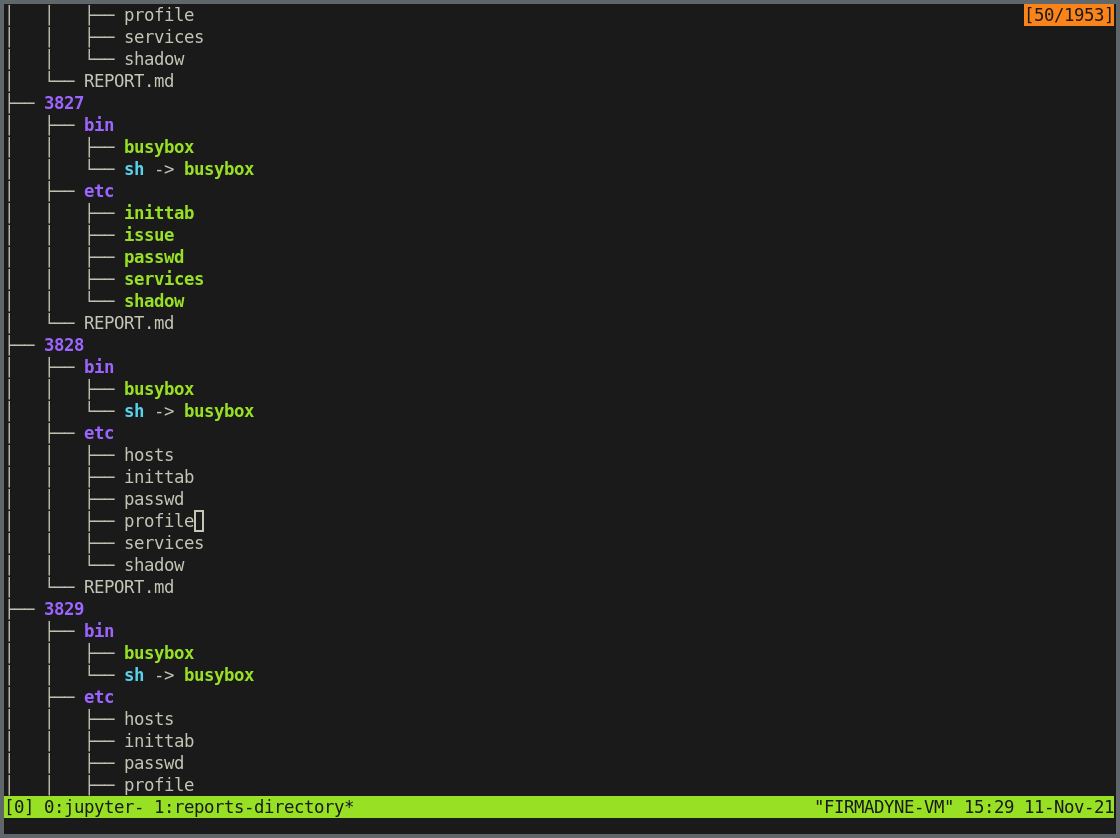
\includegraphics[width=0.65\textwidth]{figs/tree.png}
    \caption{Structure of the directory containing extracted firmware interesting files and the generated report for each firmwre.}
    \label{fig:reports-directory}
\end{figure}

This structure was designed because in the same time that it is difficult to visually extract useful information from a large compilation of exposed firmware files together from a whole database of firmware images, it may be very useful for a security specialist to have separated the interesting files for a given firmware target. This way, if a professional wants to analyse the interesting files for a given firmware, he can easily browse the reports directory and search for the directory matching the ID of the target firmware.

More than that, this structure makes it easy to automatically generate pretty formatted reports of information for a given firmware target, and that is exactly what we implemented next.

Beyond automatically generating reports, saving the interesting firmware exposed files in a specific directory allows for batch processing and data mining in the whole dataset of exposed files for all extracted firmware exposed filesystems. This idea was not implemented in this work, but can be implemented in the future during the Clustering phase of the SCREEN project. The result of the mentioned analysis could find common hashes or common configuration files containing unsafe parameters.

\subsection{Automatically Generated Reports}
\label{sec:auto-reports}

Using the code implemented in Section \ref{sec:firmware-content-statistics}, we then implemented a tool to automatically produce reports containing firmware information and interesting exposed files content for each firmware.

The reports were produced in raw text files using the Markdown language format. This way, a Markdown visualization software can be used to print the report in a beautiful processed way. In our repository \cite{github:c2dc-toso} we implemented a notebook to automatically produce the automatic reports for given firmware targets and also a notebook to visualize produced reports (after markdown compilation) for given target firmware targets.

Figure \ref{fig:automatic-report} shows the look of the first page of the report that was automatically produced for the firmware with ID = 11. If a security specialist wants to analyse the security of a specific router firmware, the produced report can serve as a starting point to the specialist.

\begin{figure}[H]
    \centering
    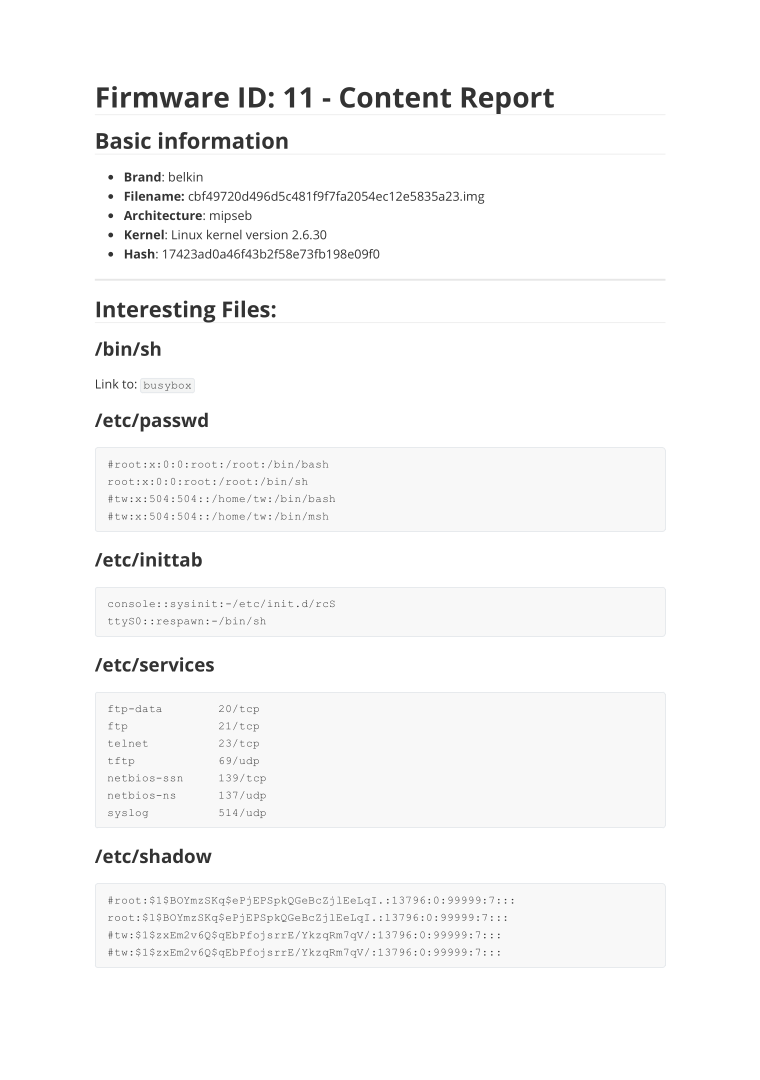
\includegraphics[width=0.75\textwidth]{figs/REPORT2.png}
    \caption{First page of a produced report in Markdown format for a given firmware target (in this case firmware with ID = 11).}
    \label{fig:automatic-report}
\end{figure}

Some examples of exposed interesting files we decided to include in the generated reports and the number of firmware images exposing these files are illustrated in Table \ref{tab:exposed-files}

\begin{table}[H]
\centering
\caption{Exposed interesting files found in firmware filesystems and included in the generated reports.}
\resizebox{\textwidth}{!}{\begin{tabular}{ccc}
\hline
\textbf{File}                           & \textbf{Description}                                                                   & \textbf{Number of files} \\ \hline

{\tt /etc/profile} or {\tt /profile}    & {\footnotesize System wide environment variable definitions.}                                                                                                    & 1505      \\

{\tt /etc/passwd} or {\tt /passwd}      & {\footnotesize \begin{tabular}[c]{@{}c@{}}File containing user login accounts (usernames),\\ default home directory and shell for each user.\end{tabular}}       & 1502      \\

{\tt /etc/inittab} or {\tt /inittab}    & {\footnotesize Init daemon configuration.}                                                                                                                       & 1057      \\ 

{\tt /etc/shadow} or {\tt /shadow}      & {\footnotesize Password hashes for system's account.}                                                                                                            & 912       \\

{\tt /etc/ssh/ssh\_host\_key}           & {\footnotesize \begin{tabular}[c]{@{}c@{}}Private SSH key\\(Security Critical - Should not be exposed).\end{tabular}}                                            & 13        \\

{\tt /etc/ssh/sshd\_config} or {\tt /etc/sshd\_config} 
                                       & {\footnotesize SSH daemon configuration files.}                                                                                                                   & 6        \\ 

{\tt /etc/ssh/ssh\_config} or {\tt /etc/ssh\_config} 
                                       & {\footnotesize SSH client configuration files.}                                                                                                                   & 5        \\ \hline
\end{tabular}}
\label{tab:exposed-files}
\end{table}

Particularly the exposed private SSH keys are security critical. Depending on how this SSH key is used by the products in question, if any device is configured to trust the public key associated with the exposed private SSH key, the content of the private key is enough to give an attacker free SSH access to a target. Note that this exposed files search was simply conducted searching for specific files in common directories. If we implement a more advanced search (e.g search by file contents) we could possibly discover even more private SSH keys and credentials exposed in our firmware dataset.

Also, we investigated what is the default shell used in the firmware images. As it is commom for embedded devices, our intuition pointed that the default shell for the extracted firmware images would probably be the {\tt busybox} shell. Our investigation confirmed this intuition: From the 1279 identified shells for the extracted firmware, $96.60\%$ ($1208$) were {\tt busybox} shells and $5.40\%$ (69) were {\tt bash} shells, as shown in Table \ref{tab:shell-count}.

\begin{table}[H]
\centering
\caption{Identified shells in extracted firmware filesystems.}
\begin{tabular}{cc}
\hline
\textbf{Shell} & \textbf{Number of Identified Shells} \\ \hline
{\tt busybox}        & 1208 (94.60\%)              \\
{\tt bash}           & 69 (5.40\%)                 \\ \hline
\end{tabular}
\label{tab:shell-count}
\end{table}

A recent post made by the cybersecurity team Claroty’s Team82 in partership with JFrog (a company that develops lead solutions for DevOps and software updates management) claims that they made the discovery of 14 vulnerabilities inside the {\tt busybox} software. The registered CVE's for each vulnerability suggests that these vulnerabilities allows for Denial of Service (DoS) and possible Remote Code Execution (RCE)~\cite{jfrog-busybox}. As shown by Table \ref{tab:shell-count}, the vulnerabilities in {\tt busybox} discovered by Claroty and JFrog are of great concern because most home wireless routers installed today may have vulnerable {\tt busybox} binaries and this could be another source for a large scale network attack. Because these vulnerabilities in {\tt busybox} were so recently disclosed, there were no able time to explore them. In future works, investigating the published CVE's for {\tt busybox} may be a great idea. More about future work suggestions in Section \ref{sec:future-work}.

\section{Kernel Cross-compilation \& Toolchain Building}

As shown by Table \ref{tab:kernel-family-stats}, kernel family 2.6 was the second most commonly found amongst successfully extracted kernels and is a very kernel family (the longest supported 2.6 kernel ended it's life in 2016 although there is still one 2.6 kernel - 2.6.32 - that is still being maintained by Canonical Ltd.\footnote{\url{https://en.wikipedia.org/wiki/Linux_kernel_version_history}}). Therefore, we investigated the difficulties of cross-compiling a 2.6 Linux kernel. At first, we tried to cross-compile the kernel in a raw modern operating system. We chose Debian 10 (running with Linux kernel version 4.19) as the starting point for this experiment. In this environment, with {\tt gcc} version 8.3.0 as the compiler and using {\tt libc} version 2.28.10 it was not possible to compile the target kernel.

Then we downloaded an old version of the Debian operating system, with a release date similar to the 2.6 Linux kernel. Debian 3.1r8 (kernel 2.4.27) was used for this experiment. Using this old operating system, with {\tt gcc} version 3.3.5 as the compiler and using {\tt libc} version 2.3.2, we had success in compiling the target kernel.

This highlights the impact the toolchain (compiler, binary utilities and library versions) has on kernel compiling process and therefore to achieve a way to automate kernel compiling, we also need a way to automate toolchain building. In this context, we adopted the {\tt crosstool-ng} tool. With this program, the user can define, between some pre-configured settings, specific versions for each tool inside the toolchain, and the program then tried to compile the desired toolchain.

Using {\tt crosstool-ng} we were then able to successfully compile a 2.6 Linux kernel inside a Debian 10 (modern operating system). However, when trying to cross-compile the target kernel for the {\tt MIPS} architecture (cross-compiling), we still faced issues that did not allow the kernel to compile successfully and further investigation is needed in order to build a working toolchain for this scenario.

\section{Firmware Re-hosting}

Regarding firmware re-hosting, in this section we will describe our team efforts towards re-hosting firmware images using the projects mentioned in the related work session.

\subsection{Manual Re-hosting}
\label{sec:manual-rehosting}

Before evaluating the performance of automated tools in the process of re-hosting firmware, to better understand how the QEMU tool can be used to boot and emulate a system, we first investigated how to manually re-host a firmware configuring QEMU in system mode emulation and preparing a firmware image to be re-hosted. In it's work, \cite{victor-sales} the fundamentals for manually re-hosting a donwloaded firmware image and presents it's results while emulating two different firmware images from wireless routers.

In \cite{victor-sales} work, re-hosting is done in a very similar approach with the one taken by Firmadyne~\cite{firmadyne} authors, in which firmware kernel is replaced with a pre-compiled similar Linux kernel, and then QEMU is used in system mode to boot the custom kernel. \cite{victor-sales} uses a pre-compiled Linux kernel version 2.6.35 with a minimal filesystem to boot a firmware and leverage QEMU network capabilities to bridge the host operating system and the system emulated with QEMU. After that, he uses the {\tt scp} utility (a command line tool to copy files using the SSH protocol) to copy the contents of the original firmware filesystem to the re-hosted operating system running with QEMU.

We decided to follow the steps described for this ``manual'' firmware re-hosting to gain more understanding of the process. The firmware with ID = 11 was randomly selected to be manually emulated. Before executing the steps to emulate the firmware with QEMU, reading the automatically generated report we implemented in Section \ref{sec:auto-reports} can already provide us with useful information about the firmware we want to re-host. Image \ref{fig:automatic-report} already shows the first page of the report generated for the firmware with ID = 11 (our target firmware in this experiment). From the first page of the report we generated automatically we already have the pieces of information required for starting the manual re-hosting:

\begin{itemize}
    \item Firmware arquitecture is MIPS Big Endian ({\tt mipseb}): We shall use the {\tt qemu-system-mips} to translate this firmware binaries correctly.
    \item Firmware original kernel is Linux version 2.6.30.
    \item The {\tt /etc/inittab} file from this firmware is exposed and from it's content we have the lead that the {\tt /etc/init.d/rcS} file from this firmware filesystem has the basics instructions of this router operation.
\end{itemize}

We then downloaded a basic Debian kernel version 2.6.32 (close to our target kernel version) and filesystem from a pre-compiled binary provided on the Debian project website\footnote{https://people.debian.org/~aurel32/qemu/mips/}. Following the instructions provided~\cite{victor-sales} the basic firmware boot consisted of executing the command shown in Code \ref{code:qemu-manual}.

\begin{listing}[!ht]
\inputminted[fontsize=\footnotesize,breaklines]{text}{Code/qemu-manual}
\caption{Command line to start QEMU in system mode running a minimal Debian running in MIPS architecture.}
\label{code:qemu-manual}
\end{listing}

This causes QEMU to open a window in which we can see the emulation of a screen connected to the firmware being re-hosted. As shown by Figure \ref{fig:qemu-manual}, the basic Debian kernel boots successfully using QEMU on system mode.

\begin{figure}[H]
     \centering
     \begin{subfigure}[b]{0.45\textwidth}
         \centering
         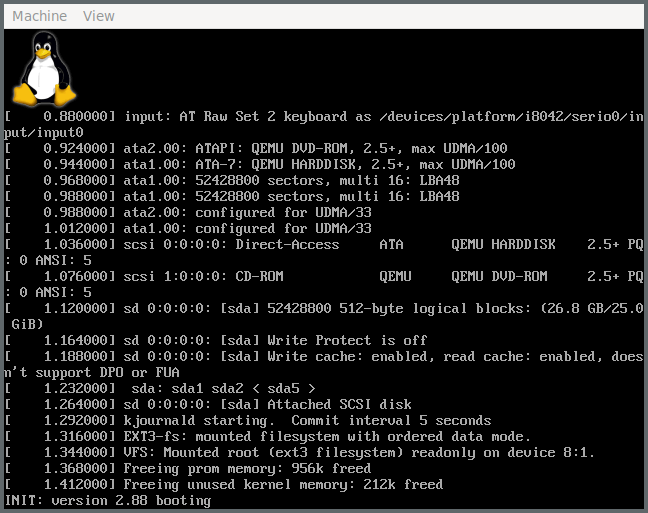
\includegraphics[width=\textwidth]{figs/qemu.png}
         \caption{Booting in process.}
         \label{fig:qemu-loading}
     \end{subfigure}
     \hfill
     \begin{subfigure}[b]{0.45\textwidth}
         \centering
         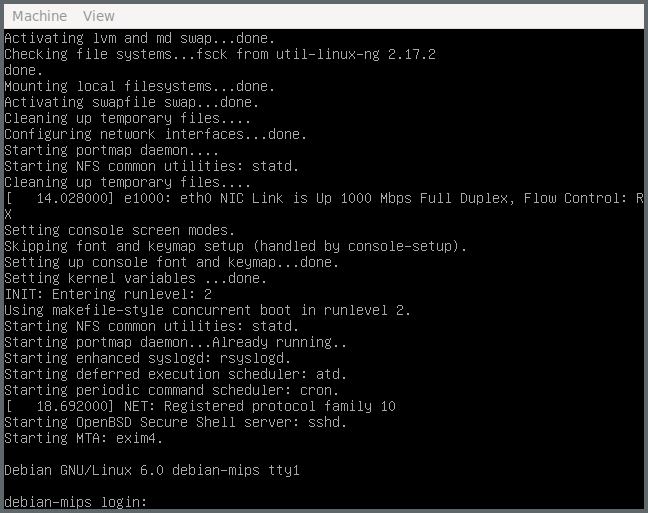
\includegraphics[width=\textwidth]{figs/qemu2.png}
         \caption{Boot completed.}
         \label{fig:qemu-booted}
     \end{subfigure}
        \caption{QEMU running on system mode emulating a Linux running on MIPS architecture.}
        \label{fig:qemu-manual}
\end{figure}

After the system has booted, we copied the original firmware filesystem contents into the emulated system using the {\tt scp} utility and rebooted the emulated system. After rebooting the firmware, with the original firmware contents in the filesystem, the boot process was not successful. This result was already expected based on what was reported by Sales~\cite{victor-sales} experiments.

\begin{figure}[H]
     \centering
     \begin{subfigure}[b]{0.45\textwidth}
         \centering
         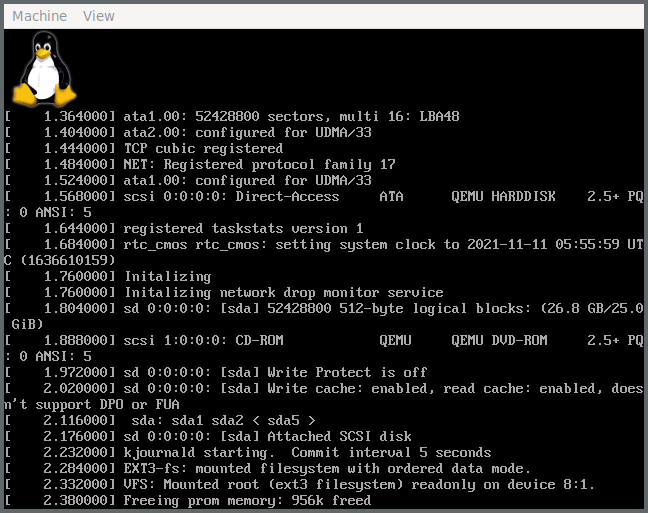
\includegraphics[width=\textwidth]{figs/qemu3.png}
         \caption{Booting in process.}
         \label{fig:qemu-loading}
     \end{subfigure}
     \hfill
     \begin{subfigure}[b]{0.45\textwidth}
         \centering
         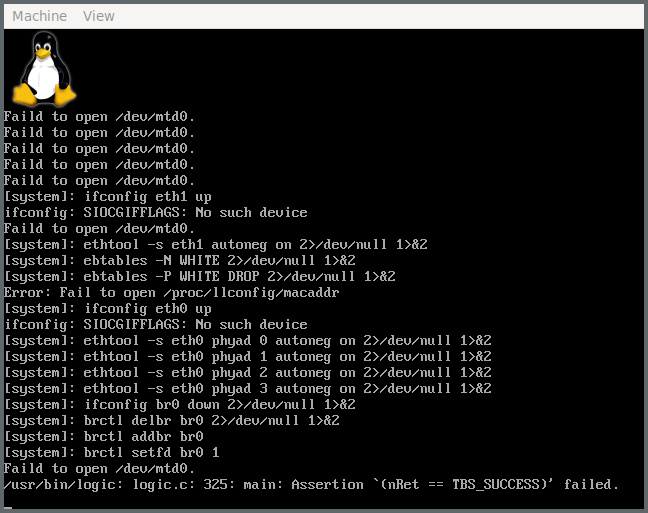
\includegraphics[width=\textwidth]{figs/qemu4.png}
         \caption{Failures during boot process (Boot not completed).}
         \label{fig:qemu-booted}
     \end{subfigure}
        \caption{Failure in the booting process after overwriting the emulated filesystem with the original firmware filesystem.}
        \label{fig:qemu-manual-error}
\end{figure}

Next we followed the approach of reading the contents of the most prominent files loaded by the {\tt /etc/inittab} and try to at least emulate the most simple firmware behavior. Inspecting the {\tt /etc/init.d/rcS} file, we discover that this file loads a lot of other files. Inspecting each of the loaded files, we discover that the {\tt /etc/init.d/daemon.rc} file loads the web server behavior of the router. Code \ref{code:daemon.rc} shows the header of the {\tt /etc/init.d/daemon.rc} file.

\begin{listing}[!ht]
\inputminted[fontsize=\footnotesize]{bash}{Code/daemon.rc}
\caption{Header of the {\tt /etc/init.d/daemon.rc} file.}
\label{code:daemon.rc}
\end{listing}

This gives us an insight about this firmware's basic functionality. It uses the {\tt mini\_httpd} binary to host a Web Server and serves the {\tt /usr/www} directory. We were not successful when trying to execute the {\tt mini\_httpd} binary inside the emulated environment. It seems that the binary headers of the {\tt mini\_httpd} binary copied to the emulated machine had corrupted headers (error accused by the {\tt file} command inside the virtual system). As emulating firmware behavior individually is not the goal of our work, we ended the ``manual re-hosting'' here, as - although the firmware was not completely emulated - the experiment was already sufficient to provide valuable insights about the re-hosting process and router firmware behavior.

\subsection{Re-hosting via Firmadyne}

Firmadyne provides scripts that can produce a {\tt QEMU} compatible disk from a firmware filesystem (that was previously extracted) applying some tweaks and patches in the filesystem of this produced disk. For instance the script replaces the {\tt busybox} binary with a statically-compiled version, replaces the password of the root user, guarantees that the filesystem contains some critical files, replaces the NVRAM library and many other minor tweaks.

This is already a great advantage when compared to the manual re-hosting described in Section \ref{sec:manual-rehosting}, because when manually copying the filesystem with the {\tt scp} utilities, we faced error that prevented the firmware to sucessfully reboot. Firmadyne~\cite{firmadyne} implementation uses this approach of creating a system disk based on the original firmware filesystem and applying patches to fix the firmware boot (like the NVRAM patch). If a firmware boots successfully, it's execution fidelity is considerably greater than the one we can have when emulating the firmware behavior simply by copying the most critical files served by the HTTP server.

% ==========================================================================================================

The first experimentation with re-hosting via Firmadyne was to try to perform the re-hosting of at least one firmware by manually executing Firmadyne's instructions one by on.e Selecting at random three firmware images that were successfully extracted and had the kernel version and architecture detected we made the first re-hosting experiments using the scripts provided by Firmadyne. The three selected firmware images on this steps were from the vendors Netgear, Belkin and Buffalo, executing Linux kernel version {\tt 3.14.4} ({\tt ARM}), {\tt 2.6.30} ({\tt MIPS}) and {\tt 3.10.1} ({\tt MIPS}) respectively.

While trying to re-host the selected firmware files with Firmadyne, only the Netgear firmware had its network interface successfully detected before the actual re-hosting. Table \ref{tab:fist-rehosting} shows the first results when trying to execute the Firmadyne's re-hosting capabilities for the three selected firmware images mentioned in the previous paragraph.

\begin{table}[H]
\centering
\caption{First results when experimenting with Re-hosting via Firmadyne. Firmware images selected at random. Minimal Firmadyne automation involved.}
\begin{tabular}{cccccc}
\hline
\textbf{Firmware ID} & \textbf{Vendor} & \textbf{Architecture} & \textbf{Kernel} & \textbf{Network Interface} & \textbf{Result} \\ \hline
2                    & Netgear         & {\tt ARM}                   & {\tt 3.14.4}                  & {\tt 192.168.1.250}                       &  Sucess                          \\
11                   & Belkin          & {\tt MIPS}                  & {\tt 2.6.30}                 & Not Detected                        &    Network Error                       \\
48                   & Buffalo         & {\tt MIPS}                 & {\tt 3.10.1}                 & Not Detected                        &        Kernel Panic                    \\ \hline
\end{tabular}
\label{tab:fist-rehosting}
\end{table}

After blindly trying to execute Frimadyne's re-hosting capabilities and failing, we then tried to better understand the tool by extensively reading it's code. Analysing Firmadyne's repository one can see that if does three basic steps in order to try the re-hosting of a well extracted and known firmware image (Firmadyne does not perform these steps atuomatically. The user has to execute then in order manually):

\begin{enumerate}
    \item For one extracted firmware filesystem, build a QEMU disk (emulates the disk image of a hard drive) applying the filesystem patches to bypass firmware peripherals dependencies. This process is costly and slow, because it requires to uncompress the firmware filesystem (saved in a directory inside our project), create a virtual partition using {\tt fdisk}, and copying the extracted filesystem to this new partition, saving it to a file and storing it in a directory that is designed to hold these generated QEMU disks. This is done by the {\tt makeImage.sh} script from Firmadyne repository.
    
    \item For a already build QEMU disk, Firmadyne then tries to infer which network ip address this router would probably use. This is done by starting a process similar to the final process of re-hosting. QEMU is started on system mode with the same exact command to be used in the next step to perform the final re-hosting of the firmware, but with a timeout of 60 seconds. During these 60 seconds the firmware is trying to boot with QEMU, Firmadyne then monitors the network interfaces of the host machine. When it detect changes in the host network, it associates this change with the firmware trying to boot within QEMU. This way Firmadyne tries to detect the interface address of the emulated firmware. This is done by the {\tt inferNetwork.sh} script from Firmadyne repository.
    
    \item Finally, the final step is to run the re-hosted firmware. This is done by simply executing the correct QEMU binary for a given architecture, and passing as a parameter to the execution of QEMU: The pre-compiled and instrumented Linux kernel (has one version if running for a MIPS architecture and one version specific for a ARM architecture), and the QEMU disk consisted of the target firmware filesystem patched with NVRAM fix, blank root password and some other tweaks. This is done by the {\tt run.sh} script from Firmadyne repository.
\end{enumerate}

